\documentclass[Softwaredesign/Softwaredesign_main.tex]{subfiles}

\begin{document}



\begin{figure}[H]
    \centering
    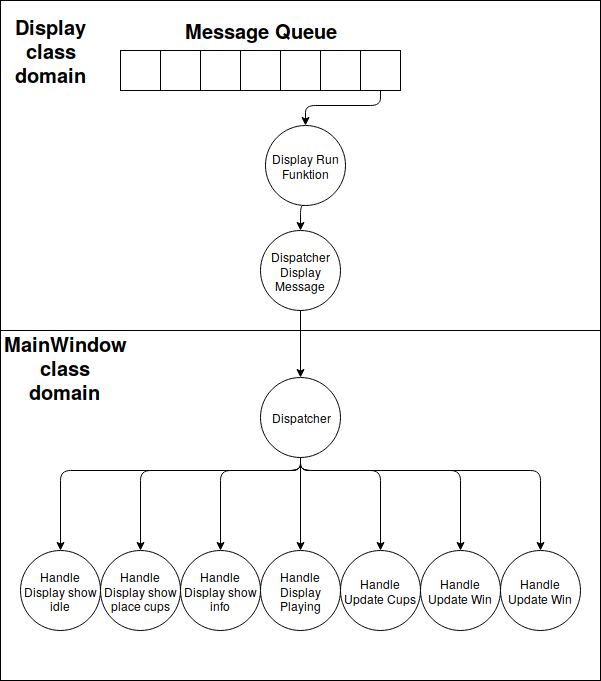
\includegraphics[scale=0.5]{Softwaredesign/GUI/Pictures/Display_MsgQ.png}
    \caption{Her ses en gennemgang af Display Message Queue}
    \label{displaymsgq}
\end{figure}

En visualiseret gennemgang af "Message Queue" systemet som bliver brugt til at sende information fra Raspberry Pi til tråden kan ses på figur \ref{displaymsgq}. Processen startes ved at der sendes en besked RPiApp som sætter en besked ind i messagen queue'en. Derefter tages besked "ud" af køen af run funktionen, som giver den beskeden videre til en dispatcher. denne dispatcher findes indenfor "Display" klassen", så den skal sendes videre til "MainWindow" domænet. Det gøres via. et funktions kald som kalder "MainWindow" klassen's dispatcher.  Denne "MainWindow" dispatcher kan så evaluerer på beskeden; alt efter besked typen: F.eks. en "Update Cups" besked, kaldes en passende "handler" funktion, som så håndtere beskeden. 
\end{document}